
\section{Introduction}
The history of neural network (NN) models have gone 
through several waves of popularity. The first 
one starts with the introduction of the perceptron
by \cite{rosenblatt1958perceptron} and its training algorithm 
for classification in linearly separable problems.
However, limitations brought up by 
\cite{minsky} somehow reduced the enthusiasm
about these models by the early 70's.
The next period of success coincides with the emergence
of results presenting NNs as universal
approximators, e.g.\ \cite{cybenko1989approximation}. Yet 
technical issues and the emergence of other paradigms like 
support vector machines led, essentially,
to a new stalmate by the early 2000's. Finally, several of the 
technical issues were solved, coinciding with the 
availability of faster computational tools,
improved algorithms and the emergence of
large annotated datasets. These produced outstanding 
applied developments leading, over the last decade, to the current boom 
surrounding deep NNs \citep{deeplearningbook}. 

This paper overviews  
recent advances in NNs. 
There are numerous reviews with various purposes
including physical \citep{cirac}, computational \citep{chollet}, mathematical \citep{maths} and statistical \citep{Banks}, 
notwithstanding  reviews concerning different  application areas 
from autonomous driving systems \citep{rumanos} to
drug design \citep{hessler}, to name but a few. 
Our emphasis is on statistical
aspects and, more specifically, on Bayesian approaches
in NN models for reasons that will become 
apparent during the presentation but include mainly:
the provision of improved uncertainty estimates, which is
of special relevance in decision support under uncertainty; their 
increased generalization capabilities; their 
enhanced robustness against adversarial attacks; 
their improved capabilities for model calibration;
and the possibility of using sparsity-inducing priors
to promote simpler NN architectures.

We first recall basic results from (the now-called) 
shallow NNs.
Section 3 then covers deep NNs, including their most
relevant 
variants, as well as classical and Bayesian approaches
for their analysis. Next, Section 4
presents three examples illustrating
diverse NN architectures. We then present 
further topics referring to security, explainability and
interpretability and transfer 
learning, and end up with a discussion.

%%%%%%%%%%%%%%%%%%%%%%%%%%%%%%%%%%%%%%%%%
\section{Shallow neural networks}
This section briefly introduces key concepts
on shallow networks to support later discussions on current approaches.
Our focus will be mainly on nonlinear regression 
problems. Specifically, we aim at approximating 
an $r$-variate response (output) $y$ with respect to $p$ explanatory 
(input) variables $x=(x_1,\ldots,x_p)$ through the 
model
\begin{eqnarray}\label{kantora}
  y         & = & \sum_{j=1}^m \beta_j \psi(x' \gamma_j) +
                    \epsilon %_i,~~i=1,\ldots,n
                    \nonumber\\
              & & \epsilon \sim N(0,\sigma^2),
                  \nonumber \\
              & & \psi(\eta) = \exp(\eta)/(1+\exp(\eta)).
                  \end{eqnarray}
This defines a neural network with one hidden 
layer with $m$ hidden neurons and logistic 
activation functions.
Figure \ref{figuradkk1} sketches 
a graphical model of a shallow NN with 10 inputs, 4 hidden nodes and 
2 outputs. 
\begin{figure}
    \centering
    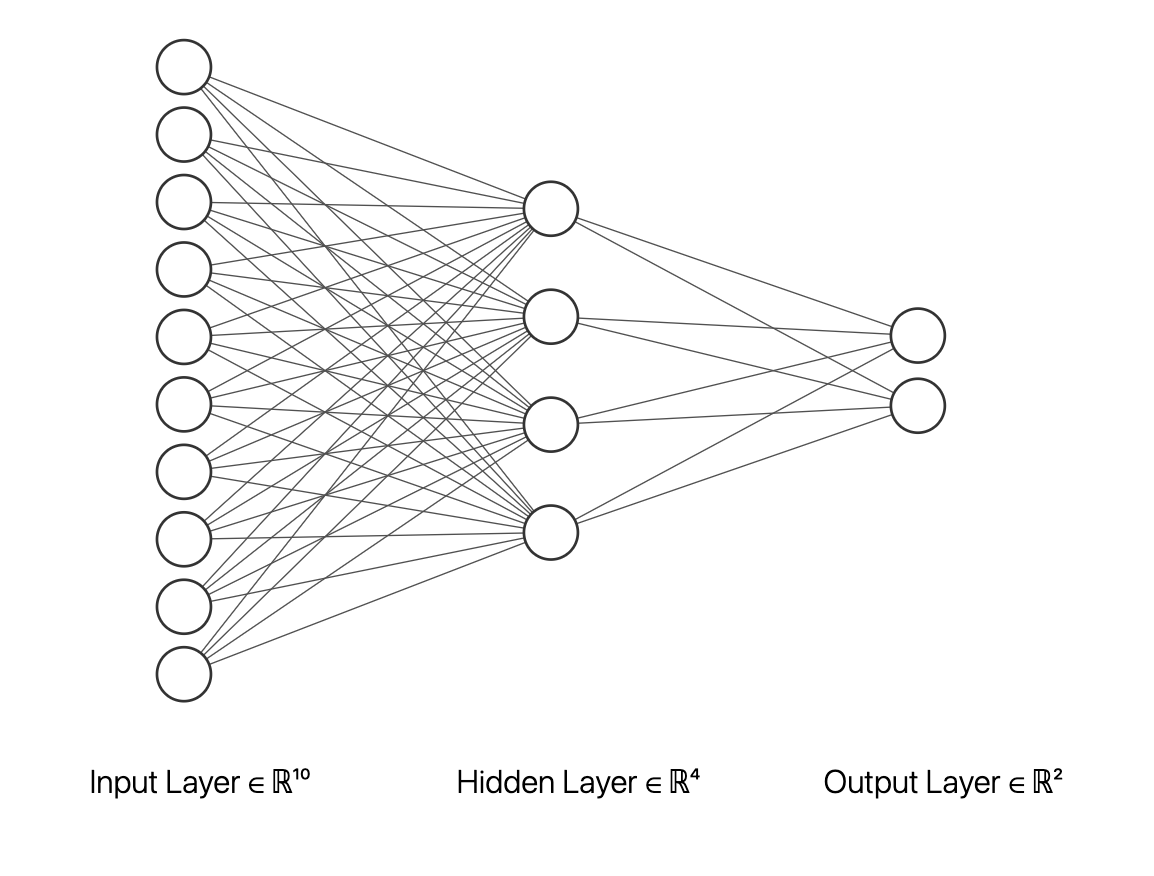
\includegraphics[scale=0.5]{figures/net1.png}
    \caption{A shallow NN architecture with 4 hidden nodes and 2 scalar outputs}
    \label{figuradkk1}
\end{figure}

Let us designate with $\beta=(\beta_1,\ldots,\beta_m)$ and $\gamma=(\gamma_1,\ldots,\gamma_m)$ the network parameters. $\sigma$  
will be considered a hyperparameter. The model
is linear in $\beta$ but non-linear in  
$\gamma$. Interest in this type of models stems from 
results such as those of \cite{cybenko1989approximation}
who presents them as universal approximators,
in the sense that any continuous function in the 
$r$-dimensional unit cube 
may be approximated by models of type
$\sum_{j=1}^m \beta_j \psi(x \gamma_j)$
when the $\psi$
functions are sigmoidal (as with the logistic) and
$m\rightarrow \infty$. Our discussion focuses on $r=1$.



%%%%%%%%%%%%%%%%%%%%%%%%%%%%%%%%%%%%%%%
\subsection{Classical approaches}\label{sanchez}

Given $n$ observations $D=\{ (x_i, y_i), i=1,...,n \}$,
 maximum likelihood estimation (MLE) 
 computes the log-likelihood and maximises it 
leading to the classical non-linear least squares problem
\begin{equation}\label{pdt}
 \min_{\beta , \gamma } f (\beta , \gamma) = \sum _{i=1}^n f_i(\beta, \gamma)  =\sum _{i=1}^n \left( y_i -
  \sum_{j=1}^m \beta_j \psi(x_i'\gamma_j) \right)^2 
 \end{equation}

\noindent Quite early, researchers paid attention to the introduction of regularisers, such as weight decay $\ell_2$ penalization \citep{krogh1992simple}, so as to improve model 
generalization, leading to the modified optimisation problem
\begin{equation}\label{kkdbak}
 \min  g(\beta ,\gamma) = f (\beta ,\gamma ) +
 h (\beta ,\gamma ), \end{equation}
where $h(\beta , \gamma )$ represents the regularisation 
term. For example, in the above mentioned case, the 
additional term is  
$h(\beta , \gamma )= \lambda _1 \sum \beta_i ^2 +
\lambda _2 \sum \sum \gamma _{ji} ^2$. 

Typically problems \ref{pdt} and \ref{kkdbak} are solved via steepest gradient descent \citep{meza} through iterations of the type
\[
   (\beta, \gamma )_{k+1}=
   (\beta, \gamma )_{k}- \eta \nabla g (  (\beta, \gamma )_{k} ),
   \]
where $\eta $ is frequently chosen as a fixed small learning rate parameter and $\nabla g $ is the gradient of the function $g$, with respect to 
$(\beta ,\gamma )$. In particular, this adopts the form 
\begin{equation}\label{gradiente1}
    \nabla g (  (\beta, \gamma )  )= \sum _{i=1}^n   \nabla f_i(\beta, \gamma) +  \nabla  h(\beta, \gamma),
    \end{equation}
    where each component of the corresponding gradients is given by 
\begin{align*}
(\nabla_\beta f_i)_k &= -2  \left(y_i - \sum_{j=1}^m \beta_j \psi(x_i' \gamma_j)\right) \psi(x_i' \gamma_k) \\
(\nabla_\gamma f_i)_{k,l} &= -2  (y_i - \sum_{j=1}^m \beta_j \psi(x_i' \gamma_j)) \beta_l \psi(x_i' \gamma_l)(1 - \psi(x_i' \gamma_l)) x_k \\
(\nabla_\beta h)_k &= 2\lambda_1 \beta_k \\
(\nabla_\gamma h)_{k,l} &= 2\lambda_2 \gamma_{k,l}.
\end{align*}

\noindent    Very importantly,  the structure of the network and the 
    chain rule of calculus %take advantage of the 
    %above structure to 
    facilitates efficient estimation of the gradients 
    via backpropagation, e.g. \cite{rumelhart1986learning}.
    
    A problem entailed by NN models in relation 
    with its estimation is the highly multimodal nature of
    the log-likelihood for three reasons:
    invariance with respect to arbitrary relabeling of
    parameters (these may
    be handled by introducing order 
    constraints among the 
    parameters);
    that inherently due to non-linearity; and, finally, 
    node duplicity (which may be dealt 
    with a model reflecting uncertainty 
    about the number of nodes,
    as explained below).
A way to mitigate multimodality is to use a global optimization method, like multistart, but
this is very demanding computationally in this domain.

Finally, note that the same kind of NN models 
may be used for nonlinear auto-regressions in
time series analysis \citep{menchero} and 
non-parametric 
regression \citep{insuamuller}. Moreover,
similar models may be used for classification purposes but this 
 requires modifying the likelihood
\citep{bishop} to e.g.\
\begin{equation}
    p(y | x, \beta, \gamma) = Mult(n=1, 
    p_1 (x, \beta, \gamma) , \ldots, p_K (x, \beta, \gamma) ),
\end{equation}
that is, one draw from a multinomial distribution with $K$ classes. 
Class probabilities
 can be computed using the softmax function,
$$
p_k = \frac{\exp{\beta_k \psi(x'\gamma_k)}}{\exp{\sum_{k=1}^K \beta_k \psi(x'\gamma_k)}}.
$$
The optimization problem is solved in a similar fashion.

%%%%%%%%%%%%%%%%%%%%%%%%%%%%%%%%%
\subsection{Bayesian approaches}\label{bayeshallow}
We discuss now Bayesian approaches to shallow NNs.
We assume standard priors 
in Bayesian hierarchical modeling, e.g.\ \citep{LavineWest}, that is,
$  \beta_i      \sim  N(\mu_\beta,\sigma_\beta^2)$
and 
  $\gamma_i     \sim  N(\mu_\gamma,S_\gamma^2)$,
  completed with priors over the hyperparameters
$\mu_\beta \sim N(a_\beta,A_\beta)$,
$\mu_\gamma \sim N(a_\gamma,A_\gamma)$,
$\sigma^{-2}_\beta \sim Gamma(c_b/2,c_bC_b/2)$,
$S_\gamma^{-1} \sim Wish(c_\gamma,(c_\gamma C_\gamma)^{-1})$ and
$\sigma^{-2} \sim Gamma(s/2, sS/2)$.
In this model, 
an informative prior probability model
is meaningful as parameters are interpretable. For example, the $\beta_ j$’s would reflect the
order of magnitude of the data $y_i$; typically positive and negative values for
$\beta _j$ would be equally likely, calling for a symmetric prior around 
0 with
a standard deviation reflecting the range of plausible values for $y_i$. Similarly,
a range of reasonable values for the logistic coefficients $\gamma_ j$ will be determined
%by the meaning of the data $y_i$ being modeled,
mainly to address smoothness
issues.

Initial attempts to perform Bayesian analysis
of NNs, adopted
arguments based on the asymptotic normality of the posterior
under appropriate conditions, as in  
\cite{mckay} and \cite{buntineweigend}. However these methods
fail if they are dominated by  
less important modes. %; moreover, some of the 
%hypothesis underlying asymptotics are doubtful 
%in the NN context.
 \cite{buntineweigend} mitigate this by finding several modes and
basing inference on weighted mixtures of the corresponding normal approximations, but we return to the same issue as some
important local modes might have been left out. An alternative view was argued
by \cite{mckay}: inference from such schemes is 
 considered as approximate
posterior inference in a submodel defined by constraining the
parameters to a neighborhood of the particular local mode. Depending on
the emphasis of the analysis, this might be reasonable, especially if in a final
implementation our aim is to set the parameters at specific values,
the usual scenario in deep learning. However,
we prefer to propagate the uncertainty in parameters, since this allows
better predictions, e.g. \citep{raftery}. 

For this, an efficient 
Markov chain Monte Carlo (MCMC) scheme
may be used \citep{muller1998issues}. It 
 samples from the posterior conditionals when available, and use
Metropolis steps, otherwise. To fight potential inefficiencies due to
multimodality, two features are built in 
 for
fast and effective mixing over local posterior modes:
whenever
possible, the weights $\gamma$ are 
partially marginalized; second,
these weights are resampled jointly.
The key observation is that,
given
the parameters $\gamma $,
we actually have a standard hierarchical normal linear
model \citep{french}. This facilitates sampling from the posterior marginals of the $\beta $ weights (step 2)
 and hyperparameters (step 4) and 
 allows marginalizing the model with respect
 to the $\beta$'s
  to obtain the marginal likelihood $p(D|\gamma, \nu)$
  (step 2), where $\nu=(\mu_\beta,\sigma_\beta,\mu_\gamma,S_\gamma,\sigma^2)$ designates the hyperparameters.
The algorithm runs like this:
{\tt 
\begin{enumerate}
  \item  Start with arbitrary $(\beta , \gamma ,\nu )$.\\
    Until convergence, iterate through 2-4
  \item  Given current $(\gamma,\nu)$, draw  
    $\beta$ from  
    $p(\beta|\gamma,\nu,y)$ (a multivariate normal).
    \item  For $j=1,...,m$,
    marginalizing in $\beta$ and given current $\nu$, draw $\gamma$ through a
    Metropolis step: \\
    Generate a candidate $\tilde\gamma_j \sim g_j(\gamma_j)$. \\
    Compute 
    $
       a(\gamma_j,\tilde\gamma_j) =
       \min\left(1,\frac{p(D |\tilde\gamma,\nu)}
                       {p(D |\gamma,\nu)}\right)
    $
    with $\tilde\gamma = (\gamma_1,\gamma_2,\ldots,\tilde\gamma_i, ...,\gamma_m)$.\\
    With probability $a(\gamma_j,\tilde\gamma_j)$ replace $\gamma_j$
    by $\tilde\gamma_j$. If not, preserve $\gamma_j$.
      \item Given $\beta$ and $\gamma$, replace $\nu$
        based on their posterior conditionals:\\
 $p(\mu_\beta|\beta,\sigma_\beta)$ is normal;
 $p(\mu_\gamma|\gamma,S_\gamma)$, multivariate normal;
 $p(\sigma_\beta^{-2}|\beta,\mu_\beta)$, Gamma; 
    $p(S_\gamma^{-1}|\gamma,\mu_\gamma)$, Wishart; 
    $p(\sigma^{-2}|\beta,\gamma,y)$, Gamma.
    \end{enumerate}
}
\noindent For proposal generation distributions $g_i(\cdot)$,
normal multivariate distributions
$N(\gamma_i,c^2 C_\gamma)$ are 
adopted. % with $c=0.1$ work in
%applications. 
Appropriate values for $c$ can be found by trying
a few alternative choices until acceptance rates around
 0.25 are achieved \citep{gamerman}. 

Combined with model augmentation to a variable architecture,
 this leads to a useful scheme
for complete shallow NN analyses as it allows for 
the identification of
architectures supported by data, by  
contemplating $m$ as an additional parameter.
A random $m$ with a prior 
favoring smaller values reduces posterior multimodality.
Moreover, as marginalization over $\gamma_ j$ requires inversion of matrices
of dimension related to $m$, 
avoiding unnecessarily large
hidden layers is critical to
reduce computational effort.
 Thus, we assume 
a maximum size $m^*$ for the network and introduce 
indicators  $d_j$ suggesting whether the node
$j$ is included ($d_j=1$) or not ($d_j=0$). 
We also 
include a linear regression term $x'a$
to favor parsimony. On the whole, the model
becomes 
\begin{eqnarray*}
  y          & = & x_i'a + \sum_{j=1}^{m^*} d_j\beta_j \psi(x '\gamma_j) +
                    \epsilon \\ %_i,i=1,...,N\nonumber\\
                    & & \epsilon \sim N(0,\sigma^2),\nonumber \\
                    & &    \psi(\eta) = \exp(\eta)/(1+\exp(\eta)),
                        \nonumber \\
  Pr(d_j=0|d_{j-1}=1)   & = & 1-\alpha, \nonumber\\
  Pr(d_j=1|d_{j-1}=1)   & = & \alpha, \nonumber\\
  \beta_i    \sim  N(\mu_b,\sigma_\beta^2),& 
  a     \sim  N(\mu_a,\sigma_a^2), &   \gamma_i   \sim  N(\mu_\gamma,\Sigma_\gamma).
                \label{eq:model-var}
\end{eqnarray*}
Learning is done through a reversible jump sampler
\citep{green} embedding our first algorithm.
As a consequence, we perform inference
about the architecture based on the distribution of 
 $p(m|D)$. 

 \cite{neal2012bayesian} proposes using an 
algorithm merging conventional Metropolis-Hastings chains with sampling
techniques based on dynamic simulation, the currently popular
Hamiltonian Monte Carlo (HMC) approaches.
Let us designate by $\theta$ the NN 
weights, $\theta = (\beta, \gamma)$, and denote the potential energy function as
$$
U(\theta) = \tau_{\beta}\sum_{i=1}^m \beta_i^2/2 + \tau_{\gamma} \sum_{i=1}^m \gamma_i^2/2 + \tau \sum_{j=1}^n (y_j - f(x_i, \theta_i))^2/2,
$$
where $\tau_{\beta}, \tau_{\gamma}, \tau$ are hyperparameters that control the amount of regularization, similarly to (\ref{kkdbak}). 
Let us also introduce the hamiltonian 
$$
H(\theta, p) = U(\theta) + \frac{1}{2} \sum_{i=1}^m p_i^2,
$$
with momentum variables $p$ of the same dimension as $\theta$; such 
 variables serve to accelerate the walk towards posterior modes. Then, the HMC scheme would be

{\tt 
\begin{enumerate}
  \item  Start with arbitrary $\theta_0 = (\beta _0, \gamma _0)$.\\
    Until convergence, iterate through 2-4
  \item  Given current $\theta_t$ and $p_t \sim \mathcal{N}(0, I)$, perform $T$ leapfrog integration
  steps 
  \begin{align*}
  p_{t + \frac{\epsilon}{2}} &= p_t - \frac{\epsilon}{2}\nabla U(\theta_t) \\
   \theta_{t+ \epsilon} &= \theta_t + \epsilon  p_{t + \frac{\epsilon}{2}} \\
   p_{t + \epsilon} &= p_{t + \frac{\epsilon}{2}} - \frac{\epsilon}{2}\nabla U(\theta_{t+ \epsilon})
    \end{align*}
    Let $\theta^*$ and $p^*$, respectively,
    be the final solution 
    and its corresponding momentum.
\item Compute $\alpha(\theta_t, \theta^*) = \min \lbrace 1, \frac{\exp H(\theta^*, p^*)}{\exp H(\theta_0, p_0)} \rbrace$
\item Accept $\theta^*$ with probability $\alpha(\theta_t, \theta^*)$, else discard it.
    \end{enumerate}
}
\noindent \cite{neal2012bayesian} also shows that,
for a broad class of priors over the parameters 
$(\beta ,\gamma )$, the distribution of functions
generated by the NN model (\ref{kantora})
will tend to a Gaussian
process as  $m\rightarrow \infty$, although, in
the limit, the output variables are independent.

%%%%%%%%%%%%%%%%%%%%%%%%%%%%%%%%%%%%%%%%
\section{Deep neural networks}

Training by backpropagation has been in use 
for many years by now.
However,
the decade of the 2010's saw major developments
leading to 
the boom over deep learning \citep{deeplearningbook}
or inference and prediction with deep NNs. 
Such advances include:
the availability of fast GPU kernels and routines
facilitating much faster training;
the access to massive amounts of data (e.g.\ Imagenet), which prevented overfitting to smaller datasets; 
the creation of new architectures, which prevented  convergence issues, such as the vanishing gradient problem; 
and the provision of automatic differentiation libraries such as Keras, Caffe or Theano.
Figure \ref{figuradkk} displays a graphical description
of what are now designated 
deep NNs, that is NNs with more than one hidden
layer, four in the portrayed case.
\begin{figure}
    \centering
    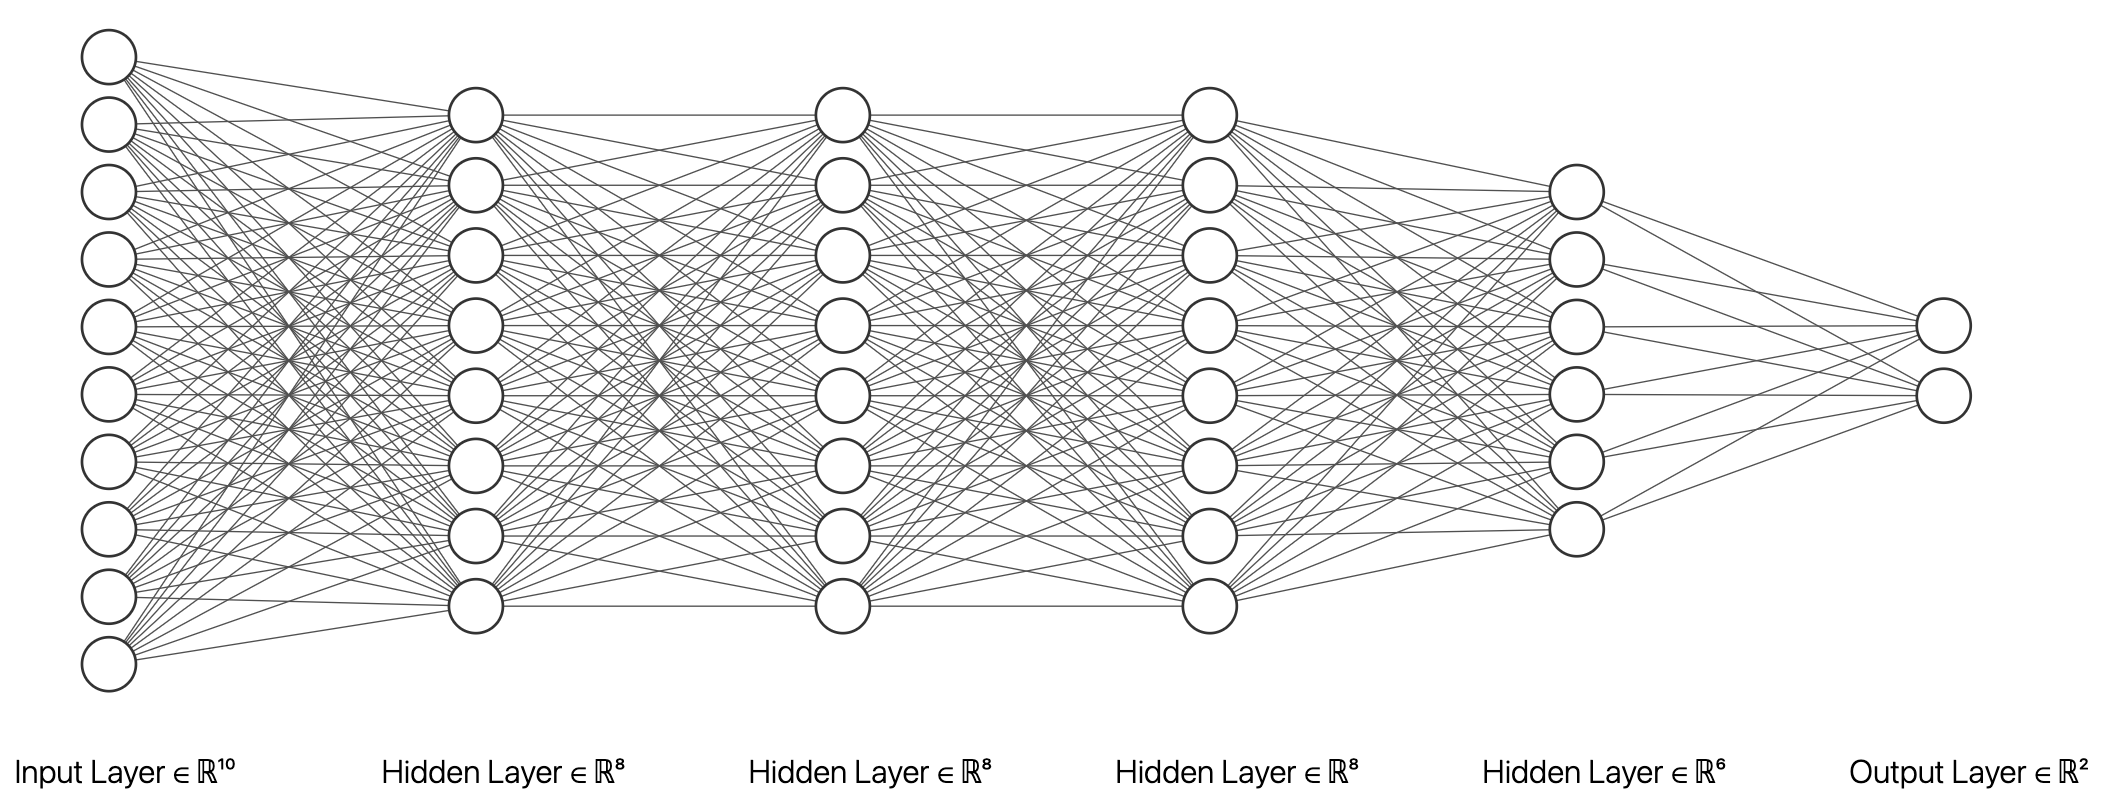
\includegraphics[scale=0.35]{figures/net2.png}
    \caption{A deep NN architecture with four hidden layers and 2 scalar outputs}
    \label{figuradkk}
\end{figure}


A deep NN may be defined through a  
a sequence of functions $\lbrace f_0, f_1, ..., f_{L-1} \rbrace$, each parametrized by some weights $\gamma_l$
of dimension $m_l$  (the corresponding number of hidden nodes) and the output of each layer being the input of the following one, as in
$$
    z_{l+1} = f_l ( z_l, \gamma_l).
$$
Lastly, we compute a prediction from the hidden activations of the last layer, as before:
\begin{eqnarray}
y         & = & \sum_{j=1}^{m_L} \beta_j z_{L,j} +
                    \epsilon %_i,~~i=1,\ldots,n
                    \nonumber\\
              & & \epsilon \sim N(0,\sigma^2),
                  \nonumber \\
\end{eqnarray}
Modern architectures do not longer require the
$f_l$ functions to be sigmoidal (like the  
logistic functions in (\ref{kantora})) and include  
the rectified linear unit (ReLU), the leaky ReLU
or the exponential LU. In particular, these functions mitigate the vanishing gradient problem \citep{kolen2001gradient} that 
plagued earlier attempts with deep architectures using sigmoidal
activation functions: recall that the derivative of the logistic function is $\psi(z)' = \psi(z)(1 - \psi(z))$, with $\psi(z) = \frac{1}{1 + e^{-z}}$; since the output of the logistic function is bounded in $\left[ 0, 1 \right]$, a concatenation of layers using this activation function makes the gradient quickly vanish to zero due to the chain rule. Alternative activation functions, such as the ReLU \citep{glorot2010understanding}, seem to alleviate this problem, in addition to having other benefits such as being faster to compute both the activation and its derivative.

%%%%%%%%%%%%%%%%%%%%%%%%
\subsection{Variants} 
Beyond the above generic deep architectures 
a few important specialised models have emerged which 
are relevant in specific application domains,
as we describe now. 
%%%%%%%%%%%%
\subsubsection{Convolutional neural networks} 
CNNs are typically used 
 in computer vision tasks and related signal processing applications.
 Stemming from the work by Le Cun and coauthors  
  \citep{lecun89, lecun98} and their original 
  LeNet5 design, they achieved major
 successes  in  competitions \citep{krizhevsky2017imagenet}
 leading to architectures like 
 AlexNet       \citep{NIPS2012_c399862d}, VGGNet \citep{simonyan2014very} or
 GoogleNet \citep{szegedy2015going}, reaching 
 superhuman performance in 
 image recognition tasks.
 
 The layer transformation is now taken to be a convolution with some 2D or 3D kernel; this makes the network able to recognise patterns independently of their location or scale in the input, a desirable property in computer vision tasks known as spatial equivariance. In addition, by replacing a fully-connected layer with a small kernel (typically, in the 2D case they are of shapes $3\times3, 5\times 5$ or $7\times 7$), there is weight sharing amongst the unit from the previous layer allows reducing 
 the number of parameters and prevents overfitting.
 
 The typical convolutional network layer is composed of several sub-layers:
 \begin{itemize}
     \item A convolution operation, as before, 
     serving as an affine transformation of the representation from the previous layer. A layer can apply several convolutions in parallel to produce a set of linear activations.
     \item A non-linear layer, such as the rectifier (based on the ReLU function), converting the previous activations to nonlinear ones.
     \item An optional pooling layer, which replaces the output of the net at a certain position with a summary statistic of 
     the nearby outputs, 
     typically the mean or the maximum.  
 \end{itemize}
 
 Note that the use of the convolution may be viewed as introducing an infinitely strong prior probability distribution over the parameters of a linear layer, in the sense that the prior places zero probability mass over certain parameters, imposing that the weights for one hidden unit must be identical to the weights of its neighbor, yet shifted in space. In a 
  similar spirit, pooling can be regarded as placing an infinitely strong prior about the function having to be invariant to small translations. If this assumption is also held in the dataset, it can vastly improve the statistical efficiency of the network.
 
 An important related development are residual networks \citep{he2016deep}, which alleviate the problem of vanishing gradients as the depth increases by also connecting the output from the previous layer to the following one, via the identity function. They thus 
 entail a residual layer of the form 
$$
z_{l+1} = f_{CNN,l}(z_l, \gamma_l) + z_l ,
$$
where $f_{CNN,l}$ is the convolutional layer at depth $l$. Current advances in CNNs aim at model scaling, suggesting that carefully balancing network depth, width, and resolution can lead to improved performance,
as with EfficientNets, \cite{tan2019efficientnet}.



%%%%%%%%%%%%
\subsubsection{Recurrent neural networks} RNNs are typically used for sequence processing, as in natural language processing (NLP), e.g.\ \cite{hochreiter1997long} and \cite{chung2014empirical}. They have feedback connections which make the network aware of temporal dependencies in the input.

Let $x_t$ denote the $t$-th token (usually a word, but can even be 
a smaller part) in the input sequence. A simple recurrent layer can be described as
$$
h_t = \psi(W_x x_t + W_h h_{t-1} + b_h)
$$
with the output at that time-step given by
$$
y_t = \psi(W_y h_t + b_y),
$$
where $\psi$ is a non-linear activation function, such as the logistic or the hyperbolic tangent functions. This is the Elman network \citep{cruse2006neural}. Note that weights are shared between different time-steps. In a similar vein to the infinitely strong prior from CNNs, this parameter sharing allows the network to search for patterns independently of their position in the sequence, yet also taking into account information from previous positions thanks to its feedback loop.

To train the previous recurrent network, all of the previous loops must be unrolled back in time, and then perform the usual gradient descent routine.
This is called \emph{backpropagation through time} \citep{58337}.
Backpropagating through long sequences may lead to the problem of vanishing or exploding gradients. Therefore, 
simple architectures like Elman's cannot be applied to longer inputs, as those arising in NLP. Gating architectures which improve the stability have been proposed and successfully applied in real-life tasks,
such as long 
short-term memory (LSTM) \citep{hochreiter1997long} and gated recurrent unit (GRU) networks \citep{cho2014learning}. 
External memory-augmented RNNs have also been proposed to tackle symbolic reasoning tasks, such as the neural Turing machine \citep{graves2014neural} or the differentiable neural computer \citep{graves2016hybrid}.

From a statistical point of view, RNNs describe directed graphical models similar to those of hidden Markov models (HMMs), but more efficiently parameterized. Assuming that each (discrete) token in the input can take $k$ different values, a HMM for sequences of length $T$ requires $\mathcal{O}(k^T)$ parameters for representing the joint distribution over the sequence; in turn, RNNs keep this requirement constant, independently of the length of the input, thanks to parameter sharing. A fruitful line of research aims to bridge the gap between classical Markov models and neural parameterizations, as in deep Kalman filters \citep{krishnan2015deep} or deep Markov models \citep{krishnan2016structured}. In the realm of memory-augmented RNNs, special attention should be given to the Kanerva machine \citep{wu2018kanerva}, a generative distributed memory updated in a Bayesian fashion.



%%%%%%%%%%%%
\subsubsection{Transformers} They substitute the sequential processing from RNNs by a more efficient, parallel approach based on attention mechanisms \citep{vaswani2017attention,bahdanau2014neural}. Their basic building components are scaled dot-product attention layers:
if $x_i$ is the embedding of the $i$-th token in an input sequence, it is multiplied by three weight matrices to obtain, 1) a query vector, $q_i = W_q x_i$; 2), 
 a key vector $k_i = W_k x_i$;
 and, 3) a value vector, $v_i = W_v x_i$. The output of the attention layer is computed, parallelizing along the input position $i$, as
$$
\mbox{softmax}\left(\frac{q k^{'}}{\sqrt{d_k}}\right) v,
$$
 a weighted average of the components of the value vector, where the average is 
computed as a normalized dot product between the key and query vectors. Thus, the attention layer produces activations for every token  that contains information not only about the token itself, but also a weighted combination of other relevant tokens weighted by the attention weights.

Each layer of a transformer model usually comprises several 
parallel layers, enabling the net to pay attention to different parts of the input simultaneously. Attention layers are alternated with  feed-forward layers in what is designated an encoder block. These 
 can be stacked until the final layer, outputting the probabilities for classification tasks. If the task requires producing outputs that are variable in length, as in automatic translation or summarization, decoder layers must be used, which replicate the work of encoders until output generation, in a similar spirit to the seq2seq models initiated a few years before with recurrent architectures \citep{sutskever2014sequence}.

Since transformer-based models are more amenable to parallelization during training, they have been trained over massive datasets in the NLP domain, leading to architectures such as Bidirectional 
Encoder Representations for Transformers (BERT) \citep{devlin2018bert}
or the series of Generative
pre-trained Transformer (GPT) models \citep{radford2018improving, radford2019language, brown2020language}. Current research avenues aim to scale transformer-based models to increasingly longer sequences \citep{tay2020long} or studying the societal and environmental issues of training gargantuan-scale models over potentially biased textual data \citep{bender2021dangers}.

From a Bayesian point of view, recent evidence suggests that transformers may be viewed as maximum 
a posteriori (MAP) estimators in 
 Gaussian mixture models \citep{movellan2020probabilistic}. Further research is necessary in this direction, since we hypothesize that the Bayesian framing may help in searching for more efficient attention kernels or the adoption of sparsity-inducing priors, which could help in keeping the size of the larger architectures under control.


%%%%%%%%%%%%%
\subsubsection{Generative models} 
This family of models, as opposed to discriminative ones, take a training set, consisting of samples from a distribution $p_{data}$, and learn to represent an estimation of that distribution, resulting in another probability distribution, $p_{model}$. Then, one could fit a distribution to the data by performing MLE,
$$
\max_{\theta} \sum_{i=1}^n \log p_{model} (x_i | \theta),
$$
or MAP estimation if a prior over the parameters $\theta$ is also placed. Fully visible belief networks \citep{10.5555/2998828.2998922} are a class of models that can be optimized this way. They are computationally tractable since they decompose the probability of any given $d-$dimensional input as $p(x | \theta) = \prod_{i=1}^d p(x_i | x_1 , \ldots x_{i-1}, \theta)$. Current architectures that fall into this category include WaveNet \citep{oord2016wavenet} and pixel recurrent neural networks \citep{pmlr-v48-oord16}. Normalizing flows can also make the distribution more flexible by means of stacking a series of suitably computable transformations \citep{pmlr-v37-rezende15}.

Another important family of models are called autoencoders \citep{autoencoders}. They perform dimensionality reduction 
using a sequence of non-linear transformations \citep{baldi2012autoencoders}: they can be regarded as a non-linear extension of principal component analysis, by stacking linear projections alternated with a non-linear activation function such as the ReLU. 
Of relevant interest are their probabilistic counterparts, variational autoencoders (VAEs) \citep{kingma2013auto}. However, these models do not have a tractable density function, and one must resort to approximation techniques. Usually, variational methods are adopted and, instead, practicioners optimize a lower bound of the model likelihood function.

In general, the term generative models 
encompasses those models and some others, such as deep Boltzmann machines or deep belief networks, see \cite{doi:10.1146/annurev-statistics-010814-020120} for a comprehensive survey.

%%%%%%%%%%%%%
\subsubsection{Generative adversarial networks} GANS  perform density estimation in high-dimensional spaces formulating a game between two players, a generator and a discriminator \citep{goodfellow2014generative}. They also belong to the family of generative models. However, GANs do not explicitly model a distribution $p_{model}$, i.e., they cannot evaluate it, only generate samples from it.
GANs define a probabilistic graphical model containing observed variables $x$ (the input data, that is an image or text) and latent variables $z$. Then, both players can be represented as two parameterized functions via NNs. Thus, the generator will be of the form $f_G(z, \theta_G)$, i.e., a NN that takes as input a latent vector and is parameterized through weights $\theta_G$. Note that the last layer will depend on the shape and range of the data $x$. Likewise, the discriminator will be a function $f_D(x, \theta_D)$, receiving a (fake or real) sample $x$ and outputting a probability for each of these two classes. Therefore, the final activation function will be 
the sigmoid or logistic function. Each network has its own objective function. For the discriminator, the cost is
$$
\mathcal{L}_G(\theta_D, \theta_G) = -\dfrac{1}{2} \mathbb{E}_{x \sim p_{data}} \log f_D(x, \theta_D) -\dfrac{1}{2} \mathbb{E}_z \log (1 - f_D(f_G(z, \theta_G), \theta_D)),
$$
that is, the standard cross-entropy for classifying real data as 1, and fake data from $G$ as 0, as for the generator objective, we could take $\mathcal{L}_D(\theta_D, \theta_G) = -\mathcal{L}_G(\theta_D, \theta_G)$,
and, consequently, both networks would play a minimax game.
Now, both players update their weights sequentially, typically using SGD or any of its variants.
However, while being helpful for theoretical analysis, 
this minimax game entails a practical problem: when the discriminator successfully rejects fake samples by the generator, since the last network is using the opposite loss function, its gradient vanishes, making the generator unable to learn how to fool the discriminator and producing better quality samples.

The vast literature on GANs is usually devoted to the previous problem. One approach to solve it is by means of heuristics. For instance, by flipping the labels for the generator, we can use as objective function
$$
\mathcal{L}_D(\theta_D, \theta_G) = -\dfrac{1}{2} \mathbb{E}_{x} \log f_D(f_G(z, \theta_G), \theta_D).
$$
More principled approaches are based on optimal transport, by minimising a Wasserstein distance between fake generated data and real data examples \citep{arjovsky2017wasserstein}. In \cite{nowozin2016f}, GANs are trained using variational divergence minimization, with the possibility of choosing any $f$-divergence \citep{CIT-004}.

While GANs have already produced astonishing results in areas such as image generation \citep{Karras2019stylegan2,brock2018large}, they are still pervaded by problems such as training instabilities or mode collapse, in which the generator gets stuck on a mode and the samples generated thus lack diversity. A probabilistic approach to deal with this problem was introduced in \cite{dieng2019prescribed}, using a regularizer based on the entropy. We expect that the adoption of methods from  Bayesian inference, such as efficient SG-MCMC samplers, may be helpful to improve the diversity of samples generated by GANs.

%%%%%%%%%%%%%%%%%%%%%%%%%%%%%%%%%%%%%%
\subsection{Classical approaches}

In principle, we could think of using 
with deep NNs the same approach as in Section \ref{sanchez}. However,
 large scale problems bring in two major
computational issues: first, the 
evaluation of the gradient (\ref{gradiente1}) 
requires going through all the $n$ observations
 becoming too expensive when $n$ is large;
second, estimation of the gradient component
for each point requires a much longer backpropagation recursion through the various levels of the
deep network, 
entailing again a very high computational 
expense. 

Fortunately, these computational demands are mitigated
through the use of classical stochastic gradient descent
(SGD)
methods \citep{robbins}
to perform the estimation \citep{bottou2010large}. SGD is the current workhorse of large-scale optimization and 
allows training deep NNs over large datasets by mini-batching: rather than going through the whole batch at each stage, just pick a small sample
(mini batch) of observations and do the corresponding
gradient estimation by backpropagation. This is reflected in the following algorithm, which departs from an
initial $\theta$.
{\tt 
\begin{enumerate}
  \item  While stopping criterion not met, do\\
  \begin{enumerate}
      \item  Sample a size $l$ minibatch 
      $((x^{(1)}, y^{(1)}),..., (x^{l},y^{l})) $
              from the training set. 
            \item Compute a gradient estimate
      $g_k = \frac{1}{l} \sum_{i=1}^l \nabla_{\theta} f_i(\theta_k) + \nabla_{\theta} h(\theta_k)$
      \item Update $\theta_{k+1} $ = $\theta_k -\epsilon _k g_k$
      \item $k=k+1$
      \end{enumerate}
          \end{enumerate}
}
\noindent The standard Robbins-Monro conditions require
that $\sum _k \epsilon_k = \infty$ and 
$\sum _k \epsilon _k^2 < \infty $ for convergence to the optimum.

Recent work has explored ways to 
speed up convergence towards the local optimum, 
leading to several variants of SGD, including the 
 addition of a momentum, as in AdaGrad, Adadelta or Adam \citep{kingma2014adam}, which we briefly review. The essence of these methods is to take into account not only a moving average of the gradients, but also an estimate of its variance, so as to dynamically adapt the learning rate. For example, in Adam, 
  parameters are updated via 
$$
\theta_{k+1} = \theta_k - \frac{\epsilon}{\sqrt{\hat{v}_k} + \eta} \hat{m}_k,
$$
where $\hat{m}_k$ and $\hat{v}_k$ are bias-corrected estimates of the gradient's mean and variance, defined as
\begin{align*}
    \hat{m}_k &= \frac{m_k}{1 - \beta_{1}} \\
    \hat{v}_k &= \frac{v_k}{1 - \beta_{2}} \\
    m_k &= \beta_1 m_{k-1} + (1 - \beta_1)g_k \\
    v_k &= \beta_2 v_{k-1} + (1 - \beta_2)g_k^2.
\end{align*}
The authors propose default values of $\beta_1 = 0.9$, $\beta_2 = 0.999$ and $\eta = 10^{-8}$, found to work well in practice.


Let us finally mention 
several techniques to improve generalization and convergence of neural networks, such as dropout \citep{srivastava2014dropout}, batch normalization \citep{ioffe2015batch} or weight initialization \citep{glorot2010understanding}.


%%%%%%%%%%%%%%%%%%%%%%%%%%%%%%%%%%%%
\subsection{Bayesian approaches}

The type of MCMC algorithms presented in Section \ref{bayeshallow}
have become standard in Bayesian inference.
 Moreover, more recent variants such as HMC
 and its Riemann
manifold variant, gain 
some efficiency of exploration, however at the cost of a significant computational burden in large datasets. Indeed, 
computing the corresponding acceptance probabilities 
 requires iterating over the whole dataset, which often does not even
 fit into memory. Thus, they 
  do not scale well to big data settings, 
 As a consequence, two major approximations have been proposed.

%%%%%%%%%%%%%%%%%%%%
\subsubsection{Stochastic Gradient Markov chain Monte Carlo}\label{bayesdeep} 

SG-MCMC methods are based on the discretization of 
stochastic differential equations that have the desired target 
distibution as its limit. \cite{ma2015complete} provide a
complete framework that encompass many earlier attempts and
facilitate such discretization as well as a practical tool for
devising new samplers and testing the correctness of proposed samplers.

Suppose as before that we aim at drawing samples from the
posterior $p(\theta |D)$. 
Let us write $p(\theta |D) \propto \exp(−U(\theta ))$,
with potential function
$U(\theta ) = −\sum {x\in D} \log p(x|\theta ) − log p(\theta )$. Define also auxiliary variables $r$ and sample from $p(z|D) \propto  exp(−H(z))$, with Hamiltonian
$H(z) = H(\theta , r) = U(\theta ) + g(\theta , r)$, such that
$\exp(−g(\theta , r))dr = constant$. (1)
Marginalizing the auxiliary variables gives us the desired distribution on $\theta $.

Generically, all continuous Markov processes that one might consider for sampling can be written
as a stochastic differential equation (SDE) of the form:
\begin{equation}
dz = f(z)dt +
\sqrt{ 2D(z)}dW(t),
\end{equation}
where $f(z)$ denotes the deterministic drift, often related to the gradient of $H(z)$, $W(t)$  is a $d$-dimensional Wiener process, and 
$D(z)$ is a positive semidefinite diffusion matrix. Note, though,
that not all choices of $f(z)$ and $D(z)$ yield the stationary distribution $p(z) \propto  exp(−H(z))$.

To devise a recipe for constructing SDEs with the correct stationary distribution, Ma et al (2015) propose 
writing
$f(z) = − [D(z) + Q(z)] \nabla H(z) + \Gamma (z)$, 
and $\Gamma _i (z) = \sum _{j=1}^d 
\frac{\pderivative}{\pderivative z_j}
D_{ij} (z) + Q_{ij} (z)$
where $ Q(z)$ is a skew-symmetric curl matrix (representing the deterministic traversing effects seen
in HMC procedures) and the diffusion matrix $D(z)$
determines the strength of the Wiener process-driven diffusion.
Both matrices can be adjusted to attain faster convergence to
the posterior distribution. When 
$D(z)$ is positive semidefinite and $Q(z)$ is skew-symmetric, we
have the convergence of the above dynamics to the desired 
distribution. Ma et al (2015) show that by properly choosing
the matrices  $D$  and $Q$ one can recover numerous samplers such
as ....

In practice, simulation relies on a discretization of the SDE, leading to the full-data update rule
\begin{equation}
z_{t+1} \leftarrow z_t - \epsilon_t [ ( D(z_t) + Q(z_t) )
\nabla H(z_t) + \Gamma (z_t)
+ N (0, 2\epsilon _t D(z_t))
\end{equation} 
Calculating the gradient of $H(z)$ involves evaluating the gradient of $U(\theta )$. With deep NN models, 
 $U(\theta )$ is very computationally intensive to compute 
 as it relies on a sum
over all data points. Instead, s
we use a sampled data subsets $S' \subset S$ and the corresponding potential for these data is
$U_1 (\theta ) = −\frac{|S'|}{|S|} \sum _{x \in S´}
\log p(x|\theta ) − \log p(\theta )$.
This leads to the approximation 
\begin{equation}
z_{t+1} \leftarrow z_t - \epsilon_t [ ( D(z_t) + Q(z_t) )
\nabla H_1 (z_t) + \Gamma (z_t)
+ N (0, \epsilon _t (2 D(z_t)- \epsilon_t \hat {B_t}))
\end{equation} 
where $\hat {B_t}$ is an estimate of the variance of the error.
This provides the  stochastic gradient—or minibatch— variant of the sampler. 

Based on this there have been seevral related particle-based approaches, such as Stein variational gradient descent (SVGD) \cite{liu2016stein}
or ****.

%%%%%%%%%%%%%%%%%%%%%
\subsubsection{Variational Bayes} 

Variational inference (VI) \citep{blei2017variational} tackles the 
 approximation of the posterior $p(\theta | D)$ with a tractable parameterized distribution $q_{\phi}(\theta |D)$. The goal is to find parameters $\phi$ so that the distribution 
$q_{\phi}(\theta |D )$  (referred to as variational guide
or variational approximation)  is as close as possible to the actual posterior, with closeness typically measured through 
the Kullback-Leibler 
divergence $KL(q_{\phi } || p)$, reformulated into the ELBO
\begin{equation}\label{eq:elbo}
\mbox{ELBO}(q) = \mathbb{E}_{q_{\phi}(\theta |D)} \left[ \log p(D,\theta ) - \log q_{\phi}(\theta |D)\right].
\end{equation}
This is the objective to be optimized,
usually through SGD techniques. 

A standard choice
for $q_{\phi}(\theta |D )$ is a factorized Gaussian 
distribution $\mathcal{N}(\mu_{\phi}(D), \sigma_{\phi}(D))$,
with  mean and covariance matrix defined through a
 deep NN conditioned on the observed data $D$.
 Note though, that 
other distributions can be adopted as long as they 
 are easily sampled and their log-density and entropy values evaluated. 
A problem is that these approximations often 
underestimate the uncertainty. Some developments
 enriching the variational family include normalizing flows \citep{rezende2015variational} or the use of implicit distributions \citep{huszar2017variational}, partly 
mitigating that issue.

We can actually use a more flexible approximation \citep{VIS},
 designated the {\em refined variational approximation}, 
  by embedding a sampler through
\begin{equation*}\label{eq:q}
q_{\phi,\eta}(\theta |D) = \int Q_{\eta, T}(\theta  | \theta _0)q_{0,\phi}(\theta _0|D)d\theta _0,
\end{equation*}
where $q_{0,\phi} (\theta | D)$ is the initial and tractable density
$q_{\phi} (\theta | D)$
(i.e., the starting state for the sampler). 
The conditional distribution $Q_{\eta, T}(\theta |\theta _0)$ refers
to a stochastic process parameterized by $\eta$,  
used to evolve the original density $q_{0,\phi}(\theta |D )$
for $T$ periods, so as to achieve greater flexibility. Specific 
forms for $Q_{\eta, T}(\theta |\theta _0)$
are described in \cite{VIS}.
 Observe that when $T=0$, no refinement steps are performed and the refined variational approximation coincides with the original one; on the other hand, as 
 $T$ increases, the approximation will be closer to the exact posterior, assuming that $Q_{\eta, T}$ is a valid sampler
 as in Section \ref{bayesdeep}.
We next maximize a refined ELBO objective, replacing in (\ref{eq:elbo}) the 
original $q_{\phi }$ 
by $q_{\phi, \eta}$
\begin{equation}\label{eq:ELBO}
\mbox{ELBO}(q_{\phi,\eta}) = \mathbb{E}_{q_{\phi, \eta}(\theta D)}
\left[ \log p(D, \theta ) - \log q_{\phi, \eta}(\theta |D)\right]
\end{equation}
to optimize the divergence $KL(q_{\phi,\eta}(\theta |D) ||  p(\theta |D ))$. 
%{\bf{The first term of Eq. (\ref{eq:ELBO})}}
%requires only being able to sample from $q_{\phi,\eta}(z|x)$; however the second
%one, the entropy
%$-\mathbb{E}_{q_{\phi,\eta}(z|x)} \left[ \log q_{\phi,\eta}(z | x) \right]$, requires also evaluating the evolving, implicit density.
%Section 3.2 describes 
Efficient methods to approximate 
 such 
evaluation are available in \cite{VIS}. As a consequence, performing variational inference with the refined variational approximation can be regarded as using the original variational guide while optimizing an alternative, tighter ELBO.  
The above facilitates a framework for learning the sampler parameters $\phi, \eta$ using gradient-based optimization, with the help of automatic differentiation \citep{baydin2017automatic}.
For this, the approach operates in two phases.
First, in a refinement phase, sampler parameters are learnt in an optimization loop that maximizes the ELBO with the new posterior;
after several iterations, the second phase,
focused on inference, starts: we just let the tuned sampler run for
sufficient iterations as used in SG-MCMC samplers. Algorithmically,
this is expressed as follows:
{\tt 
\begin{description}
    \item[Refinement phase] Repeat until convergence:
    \begin{enumerate}
    \item Sample initial set of particles, $\theta _0 \sim q_{0,\phi}(\theta | D)$.
    \item Refine particles through sampler, $\theta _T \sim Q_{\eta, T}(\theta |\theta 0)$.
    \item Compute the ELBO objective (\ref{eq:ELBO}). 
    \item Perform automatic differentiation on 
    objective wrt parameters $\phi, \eta$ to update them.
\end{enumerate}
    \item[Inference phase] Based on learnt sampler parameters $\phi^*, \eta^*$:
    \begin{enumerate}
    \item Sample an initial set of particles, $\theta _0 \sim q_{0,\phi^*}(\theta |D)$.
    \item Use the MCMC sampler $\theta _T \sim Q_{\eta^*, T}(\theta |\theta _0)$ as $T \rightarrow \infty$.
    \end{enumerate}
\end{description}
}


%%%%%%%%%%%%%%%%%%%%%%%
\subsubsection{Ensembles} \cite{bdl} shown that deep ensembles \citep{ensemble} provide an efficient technique for approximate Bayesian marginalization, but are not a truly Bayesian method.

The regularization technique called dropout can be interpreted as performing ensembling over several models \citep{dropout}. Motivated by how dropout could be effectively used to quantify uncertainty in deep networks \citep{pmlr-v48-gal16} (MC dropout), several explorations have been pursued to extend ensembles to similar purposes. Deep ensembles were found to be superior to MC dropout in out-of-distribution-settings, \cite{Ovadia2019CanYT}.
Some recent techniques that should be pointed out.
Stochastic Weight Averaging (SWA) \citep{izmailov2018averaging}, which leads to wider optima and better generalization, and a Bayesian treatment of the previous approach by fitting a Gaussian distribution, SWAG \citep{NEURIPS2019_118921ef}.

Stein Variational Gradient Descend (SVGD) \citep{svgd} takes a set of particles and evolves it following the gradient of the loss plus an auxiliary term that acts as a repulsion force between particles. Thus, the particles don't collapse into the same mode, and can explore wider areas of the posterior. There is a close relationship between SVGD and SG-MCMC methods, \citep{gallego2018stochastic} takes a step into studying the interaction between the two methods.

Deep learning ensemble applications abound, for example in probabilistic wind power forecasting \citep{wang2017deep}, speech recognition \citep{deng2014ensemble}, time series forecasting \citep{qiu2014ensemble}, and in medicine or bioinformatics \citep{qummar2019deep,xiao2018deep,cao2020ensemble}. However, the vast majority of these applied works only use simple ensembles, by averaging the outputs. Further benefits could be achieved by realizing a full Bayesian treatment of the problem.


\subsubsection{Final remarks}
Lastly, note that all of these approaches could be combined with recent heuristics to improve the convergence of stochastic gradient methods, such as the adoption of cyclical learning rates to explore more efficiently the posterior distribution over the parameters \citep{7926641}.


%%%%%%%%%%%%%%%%%%%%%
%%%%%%%%%%%%%%%%%%%%%%%%%%%%%%%%%%%
\section{Examples}
We illustrate learning with deep NNs with three examples portraying
different architectures and application domains.

%%%%%
\subsection{CNNs for image recognition}\label{kkvision}

We showcase an image classification task with a standard CNN, VGG-19, showing the superior performance compared to non-convolutional and non-deep approaches in this application domain. As benchmark, we use the CIFAR-10 dataset \citep{krizhevsky2014cifar},
which consists of 60000 32x32 colour images in 10 classes. As baselines, we use a linear multinomial regression model, and a three hidden layer MLP with 200 units each plus ReLU activations.

All models are trained for 200 epochs and minibatches of 128 samples, using SGD with a learning rate of 0.1 and  momentum of 0.9.
The learning rate is adapted with the cosine annealing scheme in  \cite{loshchilov2016sgdr}. We place Gaussian priors over all parameters (thus equivalent to $\ell_2$ regularization) and use SWA on top of the SGD optimizer, to make predictions using an ensemble of several particles, in a Bayesian way.

\begin{figure}[hbt]
\centering
  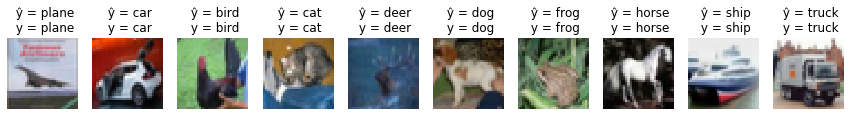
\includegraphics[width=1.\linewidth]{figures/cifar.png}
  \caption{Ten random samples from the CIFAR-10 dataset and their corresponding predictions and true labels using the VGG architecture.}
  \label{fig:cifar}
\end{figure}

Figure \ref{fig:cifar} displays ten random images from the test set.  Table \ref{tab:cnn} displays results. Notice how the linear model performs poorly, whereas increasing the flexibility of the models critically improves 
accuracy. By imposing strong priors about the dataset, such as translation equivariance thanks to the convolutional layers and pooling, state-of-the-art results can be achieved.

\begin{table}[h]
\caption{Results over the CIFAR-10 test set.}
\centering
\begin{tabular}{ll}
Model & Test acc. \\
\hline
Linear &  $38.10\%$ \\
MLP &  $50.03\%$\\
VGG-19 &  $93.29\%$ 
\end{tabular}
\label{tab:cnn}
\end{table}

%%%%%%%%%%%%%%%
\subsection{Transformer and recurrent models for sentiment analysis}
This is an example with text to undertake sentiment analysis, classifying movie reviews with architectures tailored to NLP tasks. As benchmark, we use the IMBD movie review dataset \citep{maas-EtAl:2011:ACL-HLT2011}, in which a review in raw text must be classified into one of two classes according to its sentiment: positive or negative. 

The recurrent model consists of a LSTM network with two layers, each with hidden dimension of 256 plus a dropout of 0.5 serving as a regularizer. We also consider a simple Transformer-based model, which also consists of two encoder layers, of hidden dimension 10 plus similar dropout. For both models, the input sequence is represented as a list of one-hot encoded vectors, representing the presence of a word from a vocabulary of the most common 5000 tokens. This discrete representation is embedded into a space of 100 dimensions (16 dimensions in the Transformer case) by means of an affine transformation, before applying the architecture-specific layers. Both models are trained using the Adam optimizer with a constant learning rate of 0.001.
The input sequence is represented as a list of one-hot encoded vectors, representing the presence of a word from a vocabulary of the most common 5000 tokens. This discrete representation is embedded into a space of 100 dimensions (16 dimensions in the Transformer case) by means of an affine transformation, before applying the architecture-specific layers. 
Both models are trained using the Adam optimizer with a constant learning rate of 0.001.

We also consider a bigger, Transformer-based model consisting in the recent RoBERTa architecture \citep{liu2019roberta}, which was first pretrained on a big corpus of unsupervised raw  English text, and then was finetunned for two epochs on the IMDB training set. As we will see in Section \ref{sec:transfer}, pretraining with data from different tasks or domains can crucially improve the performance of Transformer-based models, since it helps in building better representations of written language.

Table \ref{tab:examples} shows four random examples from the IMDB dataset, and results over the full test set are displayed in Table \ref{tab:nlp}. Notice how the Transformer-based models are superior to the recurrent baseline, and the extra benefits thanks to the usage of transfer learning.


\begin{table}[h]
\caption{Four random review samples and their corresponding predictions and true labels from the RoBERTa model.}
\centering
\begin{tabularx}{\textwidth}{Xll}
Text input & Prediction & True label \\
\hline
 {\scriptsize \texttt{I'm normally not a Drama/Feel good movie kind of
guy, but once I saw the trailer for "Radio", I
couldn't resist. Not only is this a great film,
but it also has grreat acting. Cuba Gooding Jr.
did an excellent job portraying James Robert
Kennedy, a.k.a. "RAdio." Ed Harris also did a
fantastic job as Coach Jones. I was pleasantly
surprised to see some comedy in it as well. So for
a great story, great acting, and a little comedy,
I give "Radio" a 10 out of 10!} } &   Positive & Positive   \\
\hline

{\scriptsize \texttt{This film was pure trash. Not the worse film ever.
If it were to be broken down, the acting was good
enough to get the job done but the script was SO
out there and so stupid that one was left
thinking, "Where did my life go?" Even Vanessa
Redgrave~ whom I love (and is the reason I watched
this) was wasted. Utterly wasted. She didn't even
leave an impression. The directing was so distant
that non of the characters left me much of
anything, but to see Redgrave leave nothing. Her
part was nothing. She was good as a mean boss but
that was it. Do depth and she's given depth to
small roles~ see Venus and Atonement. I would not
waste my time and was upset to have spent the \$5
on this movie...I wanted it back. No returns. Skip
the film. It'll only bring you grief...and
boredom.} } & Negative & Negative \\
\hline
 {\scriptsize \texttt{HOW MANY MOVIES ARE THERE GOING TO BE IN WHICH
AGAINST ALL ODDS, A RAGTAG TEAM BEATS THE BIG GUYS
WITH ALL THE MONEY?!!!!!!!! There's nothing new in
"The Big Green". If anything, you want them to
lose. Steve Guttenberg used to have such a good
resume ("The Boys from Brazil", "Police Academy",
"Cocoon"). Why, OH WHY, did he have to do these
sorts of movies during the 1990s and beyond?! So,
just avoid this movie. There are plenty of good
movies out there, so there's no reason to waste
your time and money on this junk. Obviously, the
"green" on their minds was money, because there's
no creativity here. At least in recent years,
Disney has produced some clever movies with Pixar.} } &   Negative & Negative   \\
\hline
 {\scriptsize \texttt{When I first heard that the subject matter for
Checking Out was a self orchestrated suicide
party, my first thought was how morbid, tasteless
and then a comedy on top of that. I was skeptical.
But I was dead wrong. I totally loved it. The
cast, the funny one liners and especially the
surprise ending. Suicide is a delicate issue, but
it was handled very well. Comical yes, but tender
where it needed to be. Checking Out also deals
with other common issues that I believe a lot of
families can relate with and it does with tact and
humor. I highly recommend Checking Out. A MUST
SEE. I look forward to its release to the public.} } &   Positive & Positive   \\

\end{tabularx}
\label{tab:examples}
\end{table}

\begin{table}[h]
\caption{Results over the IMDB test set.}
\centering
\begin{tabular}{ll}
Model & Test acc. \\
\hline
LSTM &  $81.99\%$ \\
Simple Transformer &  $87.49\%$ \\
RoBERTa &  $94.67\%$\\
\end{tabular}
\label{tab:nlp}
\end{table}




%%%%%%%%%%%%%%%%
\subsection{GANs for high-dimensional distribution learning}
An example in high dimensional density estimation, where we use a GAN to learn how to generate synthetic human faces with high fidelity. Concretely, we use the StyleGAN2 model from \citep{Karras2019stylegan2}. The StyleGAN family of models modifies the typical generator architecture to make it capable of unsupervised disentangling of high-level attributes (such as pose and identity in the case of human face data) and stochastic variations (such as hair or eye color) by adapting techniques from style transfer, \cite{karras2019style,jing2019neural}.







\begin{figure}[!h]
\centering
  \includegraphics[width=1.\linewidth]{figures/gan.png}
  \caption{Original image}
  \label{fig:gan}
\end{figure}






%%%%%%%%%%%%%%%%%%
\section{Other topics}
We conclude with a discussion of three transversal topics in NN
research and applications which are gaining much interest at the moment: how may we protect the predictions of deep
learning models from malicious attacks perturbing data; how can we interpret or explain the predictions of a deep model; and, finally, how may we reuse what a deep model
learns in a problem into another related context. 

%%%%%%%%%%%%%%%%%%%%%%%%%%%%%%
\subsection{Security}

As described, over the last decade
an increasing number of processes are being automated through 
deep learning algorithms, being 
essential that these are robust and reliable
if we are to
trust operations based on their output. State-of-the-art
algorithms, as those described above, perform extraordinarily well on standard data,  but have been
shown to be vulnerable to adversarial examples, data instances targeted at
fooling them \citep{goodfellow2014explaining}.
The presence of adaptive adversaries has
been pointed out in areas such as spam detection \citep{zeager2017adversarial}
and computer vision \citep{goodfellow2014explaining} among many others. 
In those contexts, algorithms should acknowledge the presence of possible adversaries
to protect from their data manipulations.
As a fundamental underlying hypothesis, NN
based systems rely on using 
independent and identically distributed (iid) data for both training and operations. However, security aspects in deep
learning, part of the emergent field of
adversarial machine learning (AML),
question such hypothesis, given the
presence of adaptive adversaries ready to  intervene in the problem 
to modify the data and obtain a benefit. 

As a motivating example, vision algorithms (Section
\ref{kkvision}) are at the core of many AI 
applications such as automated driving systems \citep{rumanos}. 
The simplest and most notorious attack examples to
such algorithms  
consist of modifications of images in such a way that the alteration becomes imperceptible to the human eye, yet drives a model trained on millions of images to misclassify the modified ones,
with potentially relevant security consequences.
With a relatively simple convolutional NN model, we are able to accurately predict 99\% of the handwritten digits in the MNIST data set.
However, if we attack those data with the fast gradient sign method \citep{szegedy2013intriguin},
accuracy gets reduced to 62\%. Fig.~\ref{fig:digits} provides an example of an original MNIST image and a perturbed one: to our eyes both images look like a 2, but the classifier rightly identifies a 2 in the first case, whereas it suggests a 7 after the perturbation. 
%
%\vspace{-0.2in}
%
%\hfill $\triangle$
%
\begin{figure}[hbt]
\centering
  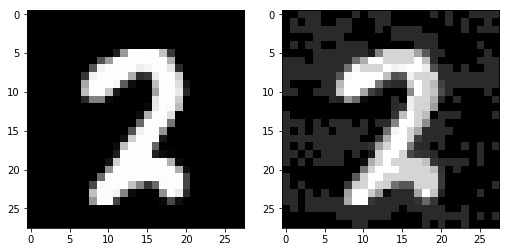
\includegraphics[width=.6\linewidth]{figures/27}
  \caption{Left: original image, correctly classified as a 2. Right: slightly perturbed image, wrongly classified as a 7.}
  \label{fig:digits}
\end{figure}

Stemming from the pioneering work in adversarial classification 
\citep{adversarialClassification2004}, the prevailing paradigm in AML models
the confrontation between learning-based systems and adversaries through game theory. 
This entails common knowledge assumptions (CK) \citep{hargreaves2004game} which are 
questionable in security 
applications as adversaries try to hide and conceal information. 
As \cite{fan2019selective} points out, there is a need for a  framework that guarantees robustness of ML against adversarial manipulations in a principled manner. 

The usual approach for robustifying models against these examples is {\em adversarial training} (AT) \citep{madry2018towards}, based on solving a 
bi-level optimisation problem whose objective function is the empirical risk of a model under worst case data perturbations. % AT approximates the inner optimisation through a projected gradient descent  
%algorithm, ensuring that the perturbed input falls within a tolerable boundary, usually specified through some restriction on a norm distance. 
However, recent pointers urge modellers to depart from using 
norm based approaches \citep{carlini2019evaluating} and develop more realistic attack models.

%Of major importance in AML is the 
%\texttt{cleverhans}\footnote{\url{https://github.com/tensorflow/cleverhans}}
%\citep{papernot2018cleverhans} library, built on top of the \texttt{tensorflow}
%framework, aimed at accelerating research in developing new attack threats and more robust defences for deep neural models.

AML is a  difficult area which rapidly evolves and leads to an 
arms race in which the community alternates cycles of proposing attacks and  of implementing defences that deal with them. However, as mentioned, it is 
based on game theoretic ideas and strong common
knowledge conditions. 
\citep{AMLARA} propose a
Bayesian decision theoretic based methodology 
to solve AML problems, 
adopting an ARA perspective \citep{adversarialRiskAnalysis2009,banks2015adversarial} modeling the confrontation between attackers and defenders and mitigating questionable CK assumptions. \citep{math8111957} applies this ARA-based framework to  adversarial classification.

%%%%%%%%%%%%%%%%%%%%%%%%%%%%%%%%
\subsection{Explainability}

Section \ref{bayeshallow} described how the parameters 
in shallow NNs remained interpretable which guided
its prior assessment. However, the complexity 
of the deep architectures in Section \ref{bayesdeep}
renders impossible both the interpretability (that is, *****) and explainability (that is, ****) of neural 
network architectures.

Predictions obtained by, e.g., artificial neural networks have a high accuracy but humans
often perceive the models as black boxes. Insights about the decision making are mostly
opaque for humans. Particularly understanding the decision making in highly sensitive
areas such as healthcare or finance, is of paramount importance. The decision-making
behind the black boxes requires it to be more transparent, accountable, and understandable
for humans.

Explainability is important in many domains but not in all domains. 
Explainability is required when there is some degree
of incompleteness. Incompleteness, to be sure, is not to be confused with uncertainty. Uncertainty refers to something that can be formalized and handled by mathematical models. Incompleteness, on the other hand, means that there is something about the problem that cannot be sufficiently encoded into the model (Doshi-Velez & Kim, 2017). For instance, a criminal risk assessment tool should be unbiased and it also should conform to human notions of fairness and ethics.

According to Lipton (2018), explainability is demanded whenever the goal the prediction model was constructed for differs from the actual usage when the model is being deployed. Explainability issues also arises for well-functioning models that fail on few data instances. Here, we also demand explanations for why the model did not perform well on these few feature combinations. According to Martens et al. (2009), explainability is essential whenever a model needs to be validated before it can be implemented and deployed. Domains that demand explainability are characterized by making critical decisions that involve, for example, a human life, e.g., in health care.
The renewed EU General Data Protection Regulation (GDPR) could require AI providers to provide users with explanations of the results of automated decision-making based on their personal data.  The GDPR may make complicated or even lead to the prohibition of the use of opaque models that are used for certain applications, e.g., for recommender systems that work based on personal data. Goodman and Flaxman (2016) call this the right of explanation for each subject (person). This will most likely affect financial institutions, social networks and the health care industry. Automated decision-making used by financial institutions for monitoring credit risk or money laundering needs to be transparent, interpretable and accountable.

Explainability and interpretability are also important aspects for deep learning models,
where a decision depends on an enormous amount of weights and parameters. Here, the parameters are often abstract and disconnected from the real world, which makes it difficult to interpret and explain the results of deep models (Angelov & Soares, 2019). Samek et al. (2017) describe different methods for visualizing and explaining deep learning models like the Sensitivity Analysis (SA) or the Layer-wise relevance propagation (LRP). Biswas et al. (2017) or Zilke et al. (2016) also mention different techniques for decompositional decision rules from ANNs.


Automated decision-making systems are not widely accepted. Humans want to understand a decision or at least they want to get an explanation for certain decisions. This is due to the fact that humans do not trust blindly. Trust, then, is one of the motivating aspects of explainability. Other motivating aspects are causality, transferability, informativeness, fair and ethical decision-making (Lipton, 2018), accountability, making adjustments and proxy functionality.


We first need to define the explanation generation process itself. While learning algorithms provide the SML model and the model, in turn, provides predictions given unseen data instances, the so-called explanator is concerned with deriving a human-comprehensible explanation for the model and/or the prediction. Thus, in any case some explanator is mandatory to gain understanding of the model used or the prediction obtained. 

There are two possible explanation generation problems: Global Extracting a global explanation from a model that is representative for some specific
data set. Local Instance explanators extract an explanation for a single test input x and the corresponding prediction y 


Learning Interpretable Models
Next, we consider models that are interpretable on their own, i.e., models that are easily comprehensible for humans. 
one aims for learning a white box model from the hypothesis
space of interpretable modelsI, which is the third way of gaining explainability.

 While using interpretable models might be appropriate for some learning problems, they come at the cost of flexibility, accuracy, and usability.
In addition, a white box surrogate model of the black box model is generated to gain
interpretability. 

We differentiate between two different kinds of surrogate models.
Global The surrogate model w approximates the black box model b on the whole training data.

Local The surrogate model approximates the black box model around a test input x
where N is some neighborhood of x.

Well-known representatives of the
class of local surrogates are LIME (Ribeiro et al., 2016c) or SHAP (Lundberg & Lee, 2017).


Rudin's paper \citep{rudin2019stop}.

Black box machine learning models are currently being used for high stakes decision-making throughout
society, causing problems throughout healthcare, criminal justice, and in other domains. People have hoped
that creating methods for explaining these black box models will alleviate some of these problems, but trying
to explain black box models, rather than creating models that are interpretable in the first place, is likely to
perpetuate bad practices and can potentially cause catastrophic harm to society. There is a way forward – it is
to design models that are inherently interpretable.








%%%%%%%%%%%%%%%%%%%%%%%%%%%%%%%%%%%%%%%%%
\subsection{Transfer learning}\label{sec:transfer}

The training of huge neural models requires large amounts of labelled data, such as images, typically in the order of thousands to millions. In cases where human labelling of the training data is not feasible to scale to those magnitudes, it is possible to leverage similar datasets, even not for the same task. This is called transfer learning \citep{tan2018survey,pan2009survey}, and fundamentally consists in taking a model previously trained over a massive dataset, and then fine-tune the model in the final task, with a much smaller dataset. The adoption of pretrained models allows the practitioner to save in computational costs, because it significantly shortens the training time for the final dataset, and often leads to improved performance, thanks to the already learnt knowledge of the pretrained model. In addition, the quantity of labelled data can be drastically reduced by strategically choosing the data points to be annotated. Techniques developed to automatize this idea fall under the term of active learning, and the Bayesian approach to statistics offers a principled and sound framework for it, see e.g. \citep{houlsby2011bayesian}.

Transfer learning has enjoyed extraordinary success in the fields of computer vision and natural language processing. With image data \citep{girshick2014rich,NIPS2014_375c7134}, it is common to pretrain a CNN on a huge dataset (typically Imagenet, \cite{deng2009imagenet}, with over 1M images from 1000 categories) and then use the CNN either an initialization (this can be regarded as specifying a Bayesian prior from the previous task) or as a feature extractor for the custom task. Typically, one removes the last layer of the pretrained CNN (the one which projects the hidden representation to the 1000 logits for Imagenet), and places another linear layer with softmax activations for the task of interest, or takes the hidden representation to use with another classifier, such as a support vector machine or a random forest, \citep{sharif2014cnn}. The Deep Image Prior is also an interesting example, as it shows that a randomly-initialized neural network can be used as a handcrafted prior with excellent results in standard inverse problems such as denoising, super-resolution, and inpainting, \cite{ulyanov2020deep}.

The case of transfer learning with textual data has gained traction more recently, with the advent of gargantuan-sized language models. Models such as BERT \citep{devlin2018bert}, or the family of GPT models \citep{radford2018improving,radford2019language,cc:BrownMannRyderSubbiahEtAl:2020:language-models}, both based on the Transformer architecture have achieved the state-of-the-art in many NLP tasks. In this case, pretraining fundamentally consists in training the Transformer to a huge amount of unsupervised data, typically scrapped from internet from sources such as Wikipedia or Common Crawl \citep{cc:BrownMannRyderSubbiahEtAl:2020:language-models}. The pretraining task is called language modeling \citep{2008SchpJ...3.3881B}: the model has to predict the next word in a sentence (causal language modeling), or fill in the gaps from a sentence with holes (masked language modeling). Then, one can replace the final layer of the Transformer encoder for a suitable task in order to perform finetuning to the desired task.

Tangential topics to transfer learning that are of increasing interest are meta-learning approaches such as model agnostic meta learning (MAML) \citep{pmlr-v70-finn17a} and its Bayesian extensions \citep{NEURIPS2018_e1021d43}. Few-shot learning \citep{wang2020generalizing}, in which a model is able to learn by providing it with only few examples per class (typically, less than 50),  has also many similitude to transfer and meta-learning. Of special interest is the extreme case of zero-shot learning, with successful applications in NLP \citep{yinroth2019zeroshot}, and computer vision, with the example of the CLIP architecture, \cite{radford2021learning}. 



%%%%%%%%%%%%%%%%%%%%%%%%%%%%%%%%%%%%%
\section{Discussion}
We end up this review by summarising results and suggesting a few challenges.
First of all, after several waves of popularity, NN models seem to 
have reached a definitive momentum because of the many relevant applications
based on them. Most work in NNs is based on the MLE tradition.
We have highlighted and illustrated the benefits of a Bayesian treatment of deep learning. To wit, they provide:
\begin{itemize}
    \item Improved uncertainty estimates, for posterior decision making.
    \item Increased generalization abilities.
    \item Increased robustness against adversaries.
    \item Improved model calibration.
    \item The use of sparsity-inducing priors.
\end{itemize}
However, efficient Bayesian integration methods in 
deep NN are 
still to be found, this remaining a major challenge.
In particular their solution would facilitate the
development of probabilistic programming 
as the next step from differentiable programming: new tools for the Bayesians of the 21st century \citep{gordon2014probabilistic,carpenter2017stan,wood2014new}.

% Summary Points
\begin{summary}[SUMMARY POINTS]
\begin{enumerate}
\item Summary point 1. Deep neural network models constitute
a major source for successful applications. 
\item Summary point 2. New NN architectures are facilitating
additional applications. 
\item Summary point 3. The prevailing paradigm is based on 
maximum likelihood plus regularisation.
\item Summary point 4. Although potentially more powerful,
Bayesian methods for deep NN still require novel efficient ideas.
\end{enumerate}
\end{summary}

% Future Issues
\begin{issues}[FUTURE ISSUES]
\begin{enumerate}
\item Future issue 1. There is a need to further develop 
large scale Bayesian methods for deep NNs.
\item Future issue 2. Security, explainability and 
interpretability of deep NNs remain as a major challenge
whose solution would facilitate wider adoption of
their models. 
\item Future issue 3. Major application areas like ADS and fake news detection demand new ideas in deep NN 
developemnts. 
\item Future issue 4. Bayesian computational developments
would lead to novel probabilistic programming environments.
\end{enumerate}
\end{issues}